\section{Data}

%\subsection{Construction of Matrix $M$}
We aim to calibrate $\alpha$ and $\beta$ for 12 categories of articles on Wikipedia (see Table \ref{tab:statistics}), as well as their evolution over 13 snapshots as presented on Figure \ref{fig:snapshots}. For each category and snapshot, we built the binary matrix $M$ by parsing all edit histories of all articles up to the snapshot time. In order to eliminate page vandals, we considered that an editor made a contribution to an article only if she has made 5 or more edits: we set $M_{ae} = 1$ for editor $e$ having modified article $a$, and $M_{ae} = 0$ otherwise. We also discarded all software robots {\it Bots}  that programmatically edit Wikipedia. 

\begin{table}
\begin{tabular}{|l|c|c|c|}
%\toprule
\hline
{\bf Category} &  {\bf Articles} &  {\bf Editors} &  {\bf Edits} \\
%\midrule
\hline
American male novelists               &      2,460 &   9,946 &  224,783 \\
2013 films                            &      1,896 &   5,215 &  150,956 \\
American women novelists              &      1,936 &   5,968 &  138,716 \\
Nobel Peace Prize laureates           &       104 &   4,165 &   91,522 \\
Sexual acts                           &        93 &   2,190 &   45,901 \\
Economic theories                     &       212 &   1,145 &   28,658 \\
Feminist writers                      &       233 &   1,357 &   25,738 \\
Yoga                                  &       123 &    730 &   25,315 \\
Military history of the US &       180 &    854 &   20,172 \\
Counterculture festivals              &        66 &    578 &   10,515 \\
Computability theory                  &        92 &    272 &    7,117 \\
Bicycle parts                         &        70 &    210 &    4,981 \\
\hline
\end{tabular}
\caption{Size statistics of investigated Wikipedia categories sorted by total edits.}
\label{tab:statistics}
\end{table}

\begin{figure}[!t]
\centering
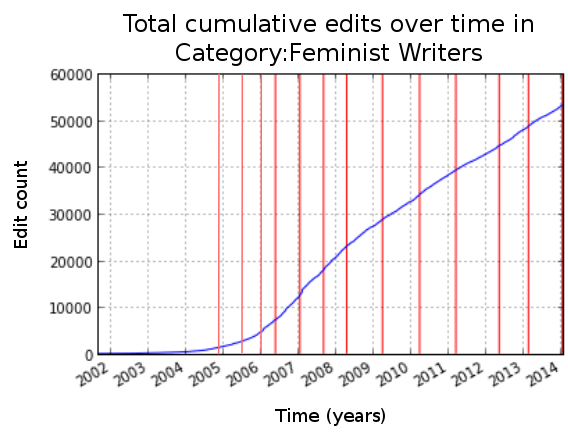
\includegraphics[width=0.9\columnwidth]{../Figures/cumulative_snapshots_Feminist_Writers_thirteen.png}
\caption{Cumulative edits made in Category {\it Feminist writers} (blue line). Vertical red lines represent the 13 snapshots taken at 2.5\%, 5\%, 7.5\% and then, 10\%, 20\%, 30\%, $...$ , 100\% of edits.}
\label{fig:snapshots}
\end{figure}

%\subsection{Editors Expertise and Articles Quality}
To calibrate $\alpha$ and $\beta$, we resorted to state-of-the-art exogenous evaluations for editor expertise $\bar{w}_e$ and article quality $\bar{w}_a$. From the exogenous evaluations, we ranked editors and articles according to their expertise and quality respectively. We then performed  a grid search for values of $\alpha^*$ and $\beta^*$, which maximize the Spearman rank-correlation $\rho_e$ and $\rho_a$ between rankings obtained from the {\it bi-partitite random walker} model $(w_e,w_a)$ and from exogenous metrics $(w_a,\bar{w}_a)$. Actually, $(\alpha^*,\beta^*)$ must maximize both $\rho_e$ and $\rho_a$, even though $rho_e$ and $\rho_a$ might actually be different. The optimization function  of $(\alpha^*,\beta^*)$ if given by,

\begin{equation}
\begin{cases}
(\alpha^*,\beta^*) = argmax(\rho_e)\\
(\alpha^*,\beta^*) = argmax(\rho_a).\\
\end{cases}
\end{equation}
$(\alpha^*,\beta^*)$ characterize how value flow from editors to articles, and conversely, in the bi-partite network of collaboration in Wikipedia.

Editors expertise is best represented by labor hours \cite{geiger2013}, and was calculated for each editor by taking contribution history up to the snapshot point. All edits made within 1 hour of a previous edit are counted in an {\it edit session}. If more than one hour separates two edits, a new edit session starts. The expertise expressed in labor hours is the sum of edit sessions. In order to capture expertise from a specific field (instead of Wikipedia editing expertise), we only consider edits for a given category. The measure of article quality is performed through a combinations of 5 text analysis metrics: (i) ratio of mark-up to readable text, (ii) number of headings, (iii) article length, (iv) citations per article length, (v) outgoing intra-Wiki links. \textcolor{red}{\bf [explain the remix version reused from \cite{klein}]}.vWe performed a Principal Component Analysis (PCA) for each category and snapshot, in order o reduce dimensionality from 5 metrics to a single one (i.e. the principal component). The variance explained by the principal component varied between 0.5 and 0.72.

